\documentclass[crop,tikz]{standalone}
\usepackage{physics}
\usetikzlibrary{positioning}

\begin{document}
% \tikzset{
%   font={\fontsize{12pt}{12}\selectfont}}
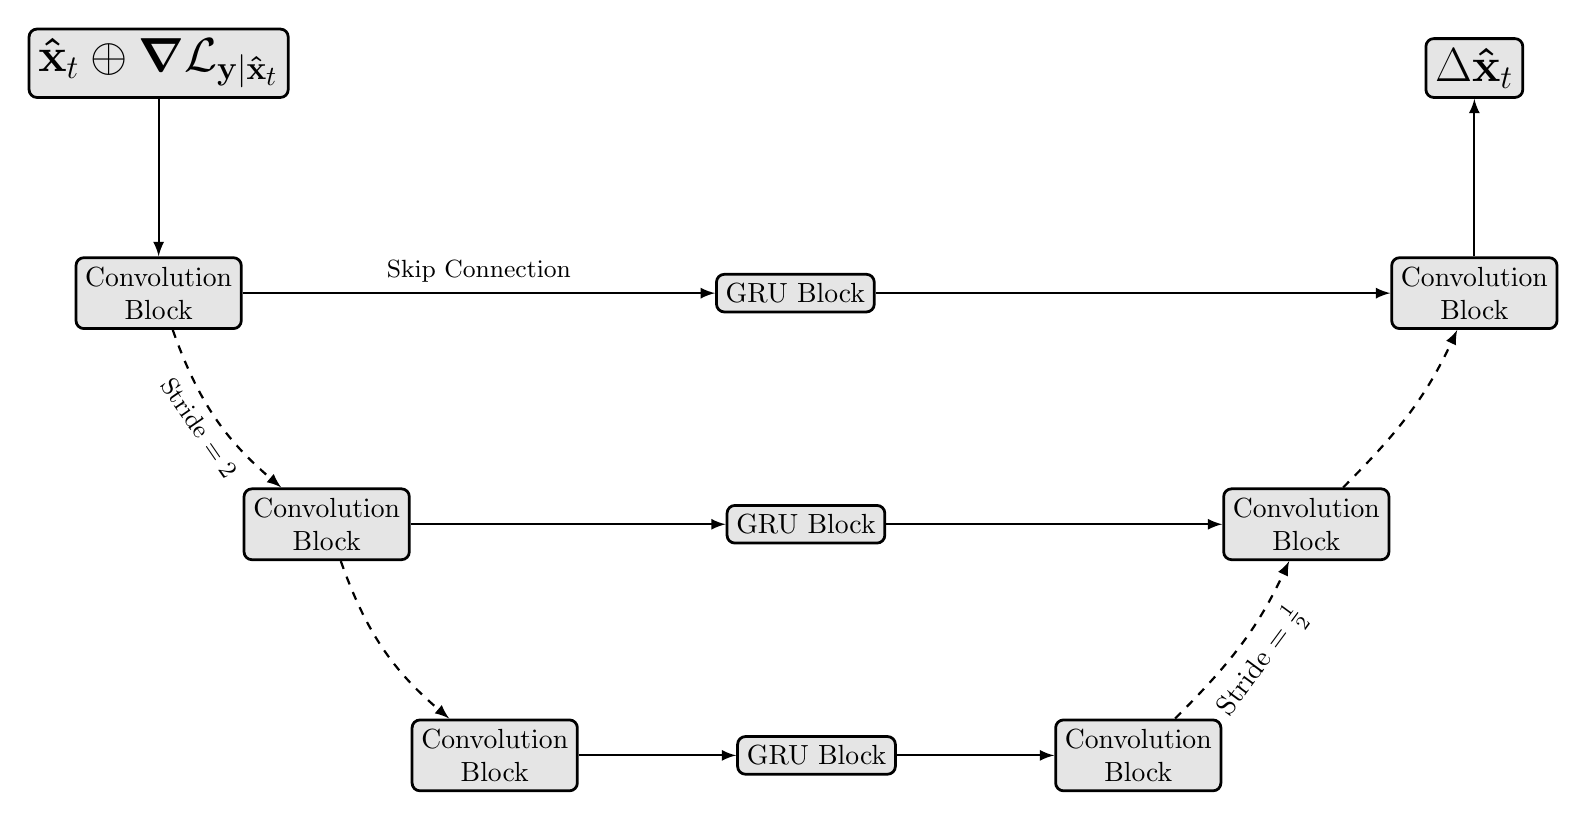
\begin{tikzpicture}[
  conv_node/.style={shape=rectangle, rounded corners=.1cm, draw=black, line width=1, fill=black!10},
  conv_node/.style={shape=rectangle, rounded corners=.1cm, draw=black, line width=1, fill=black!10},
  gru_node/.style={shape=rectangle, rounded corners=.1cm, draw=black, line width=1, fill=black!10},
  straight_edge/.style={-latex, thick},
  state_edge/.style={-latex, thick, dotted, out=245, in=160},
  state_edge_up/.style={-latex, thick, dotted, in=245, out=25},
  down_edge/.style={-latex, dashed, thick, bend right=15},
  up_edge/.style={-latex, dashed, thick, in=245, out=45},
  concat/.style={inner sep=6pt},
  node distance=3cm,
  every text node part/.style={align=center}
]
\node[conv_node] (input) at (0, 0) 
        {\LARGE$\mathbf{\hat{x}}_t \oplus \grad \mathcal{L}_{\mathbf{y} \mid \mathbf{\hat{x}}_t}$};
    
    % conv 1
    \node[conv_node] (conv1) [below=2cm of input] {Convolution \\ Block};
    \draw[straight_edge] (input) to (conv1);
    
    % conv 2
    \node[conv_node] (conv2) [below right=2cm and 0cm of conv1] {Convolution \\ Block};
    \draw[down_edge] (conv1) to node[midway, sloped, below] {\small Stride $=2$} (conv2);
    
    % Skip connection 1
    \node[gru_node] (gru1) [right=6cm of conv1] {GRU Block};
    \draw[straight_edge] (conv1) to node[midway, above] {\small Skip Connection} (gru1);
    
    
    % Skip connection 2
    \node[gru_node] (gru2) [right=4cm of conv2] {GRU Block};
    \draw[straight_edge] (conv2) to (gru2);
    
    % bottleneck
    \node[conv_node] (bottleneck) [below right=2cm and 0cm of conv2] {Convolution \\ Block};
    \draw[down_edge] (conv2) to (bottleneck);
    
    % Skip connection bottleneck
    \node[gru_node] (gru_b) [right=2cm of bottleneck] {GRU Block};
    \draw[straight_edge] (bottleneck) to (gru_b);
    
    % Upsampling conv
    \node[conv_node] (tconv1) [right=2cm of gru_b] {Convolution \\ Block};
    \draw[straight_edge] (gru_b) to (tconv1);
    
    
    \node[conv_node] (tconv2) [above right=2cm and 0cm of tconv1] {Convolution \\ Block};
    
    \node[conv_node] (tconv3) [above right=2cm and 0cm of tconv2] {Convolution \\  Block};
    
    \node[conv_node] (output) [above=2cm of tconv3] {\LARGE$\Delta \mathbf{\hat{x}}_{t}$};
    \draw[straight_edge] (tconv3) to (output);



    \draw[up_edge] (tconv1) to node[midway, sloped, below] {Stride $=\frac{1}{2}$} (tconv2);
    \draw[up_edge] (tconv2) to (tconv3);
    \draw[straight_edge] (gru1) to (tconv3);
    \draw[straight_edge] (gru2) to (tconv2);
    

\end{tikzpicture}
\end{document}
